\documentclass{article}
\usepackage[utf8]{inputenc}
\usepackage{amsmath}
\usepackage{systeme}
\usepackage{amssymb}
\usepackage[most]{tcolorbox}
\usepackage[scale=.95,type1]{cabin}
\usepackage{lmodern}
\usepackage[framemethod=tikz]{mdframed}

\usepackage{float}
\usepackage{graphicx}

\usepackage[legalpaper,margin=1in]{geometry}

\setlength{\parindent}{10pt}
\setlength{\parskip}{1em}
\renewcommand{\baselinestretch}{1.2}

\title{Linear Transformations}
\date{}

\newcounter{example}[section]
\newenvironment{example}[1][]{\refstepcounter{example}\par\medskip
   \noindent \textbf{Example~\theexample. #1} \rmfamily}{\medskip}

\makeatletter
\renewcommand*\env@matrix[1][*\c@MaxMatrixCols c]{%
  \hskip -\arraycolsep
  \let\@ifnextchar\new@ifnextchar
  \array{#1}}
\makeatother

\newcommand\y{\cellcolor{blue!10}}
\newcommand\B{\textbf}
\newcommand\tcl{\begin{tcolorbox}[colback = {blue9}]}
\newcommand\etcl{\end{tcolorbox}}

\usepackage{tabularray}
\SetTblrInner{colsep=5pt,rowsep=1pt}

\newcommand\x{\times}
\newcommand\xor{\oplus}

\makeatletter
\newcommand{\dashover}[2][\mathop]{#1{\mathpalette\df@over{{\dashfill}{#2}}}}
\newcommand{\fillover}[2][\mathop]{#1{\mathpalette\df@over{{\solidfill}{#2}}}}
\newcommand{\df@over}[2]{\df@@over#1#2}
\newcommand\df@@over[3]{%
  \vbox{
    \offinterlineskip
    \ialign{##\cr
      #2{#1}\cr
      \noalign{\kern1pt}
      $\m@th#1#3$\cr
    }
  }%
}
\newcommand{\dashfill}[1]{%
  \kern-.5pt
  \xleaders\hbox{\kern.5pt\vrule height.4pt width \dash@width{#1}\kern.5pt}\hfill
  \kern-.5pt
}
\newcommand{\dash@width}[1]{%
  \ifx#1\displaystyle
    2pt
  \else
    \ifx#1\textstyle
      1.5pt
    \else
      \ifx#1\scriptstyle
        1.25pt
      \else
        \ifx#1\scriptscriptstyle
          1pt
        \fi
      \fi
    \fi
  \fi
}
\newcommand{\solidfill}[1]{\leaders\hrule\hfill}
\makeatother

\newcommand\R{\mathbb{R}}
\newcommand\T{\textit}
\usepackage{mathtools}

\DeclarePairedDelimiter\abs{\lvert}{\rvert}%
\DeclarePairedDelimiter\norm{\lVert}{\rVert}%

% Swap the definition of \abs* and \norm*, so that \abs
% and \norm resizes the size of the brackets, and the 
% starred version does not.
\makeatletter
\let\oldabs\abs
\def\abs{\@ifstar{\oldabs}{\oldabs*}}
%
\let\oldnorm\norm
\def\norm{\@ifstar{\oldnorm}{\oldnorm*}}
\makeatother

\newcommand*{\Value}{\frac{1}{2}x^2}%
\newcommand\la{\langle}
\newcommand\ra{\rangle}

\newcommand\ddfrac[2]{\frac{\displaystyle #1}{\displaystyle #2}}

\tcbuselibrary{theorems}
\tcbuselibrary{skins}
\newtcbtheorem[]{thm}{}{
  theorem style= standard,
  enhanced jigsaw,% <--- jigsaw
  sharp corners,
  boxrule=0pt,
  toprule=1pt,bottomrule=1pt,
  left=0.2cm,right=0.2cm,top=0.2cm,
  titlerule=0em,
  toptitle=0.1cm,
  bottomtitle=0.1cm,
  colframe=white!25!black,colback=white,coltitle=black,
  title style={white!25!blue9},   %& <---- remove
  fonttitle=}{thm}

\newcounter{Lemma}[section]
\newenvironment{Lemma}[1][]{%
  \stepcounter{Lemma}%
  \ifstrempty{#1}%
  {\mdfsetup{%
    frametitle={%
      \tikz[baseline=(current bounding box.east),outer sep=0pt]
      \node[line width=1pt,anchor=east,rectangle,draw=blue!20,fill=white]
    {\strut \color{black}{\textit{THEOREM}}~};}}
  }%
  {\mdfsetup{%
    frametitle={%
      \tikz[baseline=(current bounding box.east),outer sep=0pt]
      \node[line width=1pt,anchor=east,rectangle,draw=blue!20,fill=white]
    {\strut \color{black}{\textit{THEOREM}}~:~\color{blue5}{#1}};}}%
  }%
  \mdfsetup{innertopmargin=10pt,linecolor=blue!20,%
            linewidth=1pt,topline=true,%
            frametitleaboveskip=\dimexpr-\ht\strutbox\relax,}
  \begin{mdframed}[]\relax%
  }{\end{mdframed}}

\newcounter{Def}[section]
\newenvironment{Def}[1][]{%
  \ifstrempty{#1}%
  {\mdfsetup{%
    frametitle={%
      \tikz[baseline=(current bounding box.east),outer sep=0pt]
      \node[line width=1pt,anchor=east,rectangle,draw=blue!20,fill=white]
    {\strut \color{black}{Definition}~};}}
  }%
  {\mdfsetup{%
    frametitle={%
      \tikz[baseline=(current bounding box.east),outer sep=0pt]
      \node[line width=1pt,anchor=east,rectangle,draw=blue!20,fill=white]
    {\strut \color{black}{Definition}~:~\color{blue4}{#1}};}}%
  }%
  \mdfsetup{innertopmargin=2pt,linecolor=blue!20,%
            linewidth=1pt,topline=true,%
            frametitleaboveskip=\dimexpr-\ht\strutbox\relax,}
  \begin{mdframed}[]\relax%
  }{\end{mdframed}}

\newcounter{Ans}[section]
\newenvironment{Ans}[1][]{%
  \ifstrempty{#1}%
  {\mdfsetup{%
    frametitle={%
      \tikz[baseline=(current bounding box.east),outer sep=0pt]
      \node[line width=1pt,anchor=east,rectangle,draw=blue!20,fill=white]
    {\strut \color{black}{\textit{ANSWER}}~};}}
  }%
  {\mdfsetup{%
    frametitle={%
      \tikz[baseline=(current bounding box.east),outer sep=0pt]
      \node[line width=1pt,anchor=east,rectangle,draw=blue!20,fill=white]
    {\strut \color{black}{\textit{ANSWER}}~:~\color{blue4}{#1}};}}%
  }%
  \mdfsetup{innertopmargin=2pt,linecolor=blue!20,%
            linewidth=1pt,topline=true,%
            frametitleaboveskip=\dimexpr-\ht\strutbox\relax,}
  \begin{mdframed}[]\relax%
  }{\end{mdframed}}

\newcounter{Ques}[section]
\newenvironment{Ques}[1][]{%
  \ifstrempty{#1}%
  {\mdfsetup{%
    frametitle={%
      \tikz[baseline=(current bounding box.east),outer sep=0pt]
      \node[line width=1pt,anchor=east,rectangle,draw=blue!20,fill=white]
    {\strut \color{black}{A classic problem}~};}}
  }%
  {\mdfsetup{%
    frametitle={%
      \tikz[baseline=(current bounding box.east),outer sep=0pt]
      \node[line width=1pt,anchor=east,rectangle,draw=blue!20,fill=white]
    {\strut \color{black}{\textit{ANSWER}}~:~\color{blue4}{#1}};}}%
  }%
  \mdfsetup{innertopmargin=2pt,linecolor=blue!20,%
            linewidth=1pt,topline=true,%
            frametitleaboveskip=\dimexpr-\ht\strutbox\relax,}
  \begin{mdframed}[]\relax%
  }{\end{mdframed}}


\newcounter{Conc}[section]
\newenvironment{Conc}[1][]{%
  \ifstrempty{#1}%
  {\mdfsetup{%
    frametitle={%
      \tikz[baseline=(current bounding box.east),outer sep=0pt]
      \node[line width=1pt,anchor=east,rectangle,draw=blue!20,fill=white]
    {\strut \color{blue5}{Conclude}~};}}
  }%
  {\mdfsetup{%
    frametitle={%
      \tikz[baseline=(current bounding box.east),outer sep=0pt]
      \node[line width=1pt,anchor=east,rectangle,draw=blue!20,fill=white]
    {\strut \color{black}{\textit{ANSWER}}~:~\color{blue4}{#1}};}}%
  }%
  \mdfsetup{innertopmargin=0pt,linecolor=blue!20,%
            linewidth=1pt,topline=true,%
            frametitleaboveskip=\dimexpr-\ht\strutbox\relax,}
  \begin{mdframed}[]\relax%
  }{\end{mdframed}}



\begin{document}
    \part{Introduction to Linear Transformations}
    In this chapter, we will learn about functions that \textbf{map} a vector space $V$ into a vector space $W$. 
    This type of function is denoted by 
    \[T: V \to W \]
    For instance, $V$ is called the \textbf{domain} of $T$, and $W$ is called the \textbf{codomain} of $T$.  If $\B{v} \in V, \B{w} \in W$
    such that \[T(\B{v}) = \B{w}\]
    then \B{w} is called the \textbf{image} of $v$ under $T$. The set of all images of vectors in $V$ is called the \textbf{range}
    of $T$, and the set of all \B{v} in $V$ such that $T(\B{v}) = \B{w}$ is called \textbf{preimage} of \B{w}.

   \begin{minipage}{0.6\linewidth}
       \textbf{REMARK.} For a vector $\B{v} = (v_1, v_2, \dots, v_n)$ in $\R^n$, it would be technically correct to use 
       double parentheses to denote $T(\B{v})$.

       Howerver, for convenient, one parentheses is dropped
       \[T(\B{v}) = T(v_1, v_2, \dots, v_n)\]
   \end{minipage} 
   \begin{minipage}{0.3\linewidth}
       \begin{flushright}
           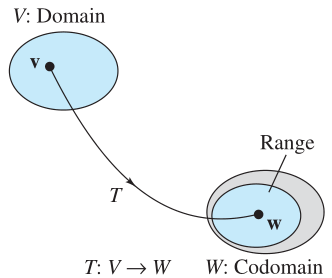
\includegraphics[width = 4cm]{images/tw1.png}
       \end{flushright}
   \end{minipage}

   \textbf{Example 1. \textcolor{blue5}{A Function from $\R^2$ into $\R^2$}}
   
   For any vector $\B{v} = (v_1, v_2)$ in $\R^2$, let $T: \R^2 \to \R^2$ be defined by
   \[T(v_1, v_2), (v_1 - v_2, v_1 + 2v_2)\]
    (a) Find the image of $\B{v} = (-1, 2)$.\\
    (b) Find the preimage of $\B{w} = (-1, 11)$.

    \textcolor{blue5}{ \textit{SOLUTION.} } (a) For $\B{v} = (-1, 2)$ you have
    \[T(-1, 2) = (-1 - 2, -1 + 2(2)) = (-3, 3)\]
    (b) If $T(\B{v}) = (v_1 - v_2, v _1 + 2 v_2) = (-1, 11)$, then 
    $\systeme {
        v_1 - v_2 = -1,
        v_1 + 2v_2 = 11
    }$

    This system of equations has the unique solution $v_1 = 3$ and $v_2 = 4$. So, the preimage of $(-1, 11)$ is $(3, 4)$.

    \begin{tcolorbox}[colback = {blue9}]
        \textbf{Definition of Linear Transformations.} Let $V$ and $W$ be vector spaces.

        The function $T: V \to W$ is called a \textbf{linear transformation} of $V$ into $W$ if
        \begin{enumerate}
            \item $T(\B{u} + \B{v}) = T(\B{u}) + T(\B{v})$
            \item $T(c\B{u}) = cT(\B{u})$
        \end{enumerate}
        for all \B{u} and \B{v} in $V$.
    \end{tcolorbox}
    A linear transformation is said to be \textit{operation preserving}, because the same result occurs whether the operations
    of addition and scalar multiplication are performed \textit{before} or \textit{after} the linear transformation is applied.
    \begin{center}
        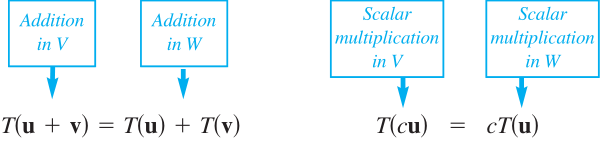
\includegraphics[width = 8cm]{images/pro1.png}
    \end{center}
    \textbf{REMARK.} A linear transformation $T: V \to V$ from a vector space \textbf{itself} is called a \textbf{linear operator}.

    \textbf{Example 3. \textcolor{blue5}{Some functions that are not Linear Transformations}}\\
    (a) $f(x) = \sin{x}$ is not a linear transformation from $\R$ to $\R$ because, in general,
    \[ \sin{x_1 + x_2} \ne \sin{x_1} + \sin{x_2}\]
    (b) $f(x) = x^2$is not a linear transformation from $\R$ to $\R$ because, in general,
    \[(x_1 + x_2)^2 \ne x_1^2 + x_2^2\]
    (c) $f(x) = x + 1$ is not a linear transformation from $\R$ to $\R$ because
    \[f(x_1 + x_2) = x_1 + x_2 + 1\]
    whereas $f(x_1) + f(x_2) = (x_1 + 1) + (x_2 + 1) = x_1 + x_2 + 2$.

    Two simple linear transformations are\\
    1. \textbf{Zero transformation} : $T(\B{v}) = \B{0},\quad \forall \B{v}$.\\
    2. \textbf{Identity transformation} : $T(\B{v}) = \B{v},\quad \forall \B{v}$.

    \begin{tcolorbox}[colback = {blue9}]
        \textit{THEOREM 6.1} \textbf{Properties of Linear Transformations}

        Let $T$ be a linear transformation from $V$ to $W$, where \B{u} and \B{v} are in $V$.
        \begin{enumerate}
            \item $T(\B{0}) = \B{0}$
            \item $T(-\B{v}) = -T(\B{v})$
            \item $T(\B{u} - \B{v}) = T(\B{u}) - T(\B{v})$
            \item If $\B{v} = c_1\B{v}_1 + c_2\B{v}_2 + \cdots + c_n\B(v)_n$, then
                \begin{equation*}
                    \begin{split}
                        T(\B{v}) &= T(c_1\B{v}_1 + c_2\B{v}_2 + \cdots + c_n\B(v)_n)\\
                                 &= c_1T(\B{v}_1) + c_2T(\B{v}_2) + \cdots + c_nT(\B{v}_n)
                    \end{split}
                \end{equation*}
        \end{enumerate}
    \end{tcolorbox}
    \textit{Property 4.} tells you that a linear transformation $T: V \to W$ is determined completely by its action on a basis of $V$.
    In other words, if $\{\B{v}_1, \B{v}_2, \dots, \B{v}_n$ is a basis for $V$, and if $T(\B{v}_1), T(\B{v}_2), \dots, T(\B{v}_n)$ is given,
    then $T(\B{v})$ is determined for \textit{any} \B{v} in $V$.

    \textbf{Example 4. \textcolor{blue5}{Linear Transformations and Bases}}

    Let $T: \R^3 \to \R^3$ be a linear transformation such that
    \begin{equation*}
        \begin{split}
            T(1,0,0) &= (2, -1, 4) \\
            T(0,1,0) &= (1, 5, -2)\\
            T(0,0,1) &= (0, 3, 1)
        \end{split}
    \end{equation*}

    Find $T(2, 3, -2)$.

    \textit{ \textcolor{blue5}{SOLUTION.} } 
    \begin{equation*}
        \begin{split}
            T(2,3,-2) &= 2T(1,0,0) + 3T(0,0,0) -2T(0,0,1) \\
                      &= (7,7,0)
        \end{split}
    \end{equation*}
    \textbf{Note.} The properties in \textit{THEOREM 6.1} provide a quick way to spot functions that are not linear transformations.

    \textbf{Example 5. \textcolor{blue5}{A Linear Transformation Defined by a Matrix}} 

    The function $T: \R^2 \to \R^3$ is defined as follows.
    \[T(\B{v}) = A\B{v} = 
        \begin{bmatrix}
            3 & 0 \\
            2 & 1 \\
            -1 & -2
        \end{bmatrix}
        \begin{bmatrix}
            v_1 \\
            v_2
        \end{bmatrix}\]
    We can use the properties of \textit{matrix multiplication} to show that $T$ is a linear transformation
    \[T(\B{u} + \B{v}) = A(\B{u} + \B{v}) = A\B{u} + A\B{v} = T(\B{u}) + T(\B{v})\]
    \[T(c\B{u}) = A(c\B{u}) = c(A\B{u}) = cT(\B{u})\]
    \begin{tcolorbox}[colback = {blue9}]
        \textit{THEOREM 6.2} \textbf{The Linear Transformation Given by a Matrix}

        Let $A$ be an $m \x n$ matrix. The function $T$ defined by
        \[T(\B{v}) = A\B{v}\]
        is a linear transformation from $\R^n$ to $\R^m$.
    \end{tcolorbox}
    
    \textbf{Example 7. \textcolor{blue5}{Rotation in the Plane}}

    \begin{minipage}{0.3\linewidth}
        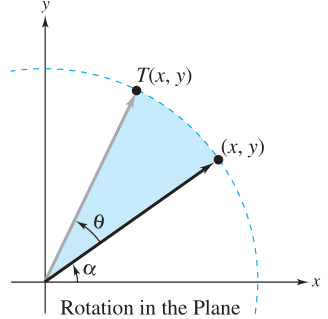
\includegraphics[width = 4cm]{images/rotate2d.png}
    \end{minipage}
    \begin{minipage}{0.6\linewidth}
            Show that the linear transformation $T: \R^2 \to \R^2$ represented by the matrix
            \[A = \begin{bmatrix}
        \cos{\theta} & -\sin{\theta} \\
        \sin{\theta} & \cos{\theta}
    \end{bmatrix}\]
    has the property that it rotate every vector in $\R^2$ counterclockwise about the origin through the angle $\theta$.

    \end{minipage}
    
    \textit{ \textcolor{blue5}{SOLUTION.} } Let $\B{v} = (x,y)$be a vector in $\R^2$. Using polar coordinates, we can write \textbf{v} as
    \[\B{v} = (x,y) = (r \cos{\alpha}, r \sin{\alpha})\]
    Now applying the linear transformation $T$ to \textbf{v} produces
    \begin{equation*}
        \begin{split}
            T(\B{v}) = A\B{v} &= \begin{bmatrix}
        \cos{\theta} & -\sin{\theta} \\
        \sin{\theta} & \cos{\theta}
    \end{bmatrix} \begin{bmatrix}
        x \\ y
    \end{bmatrix} \\
                              &= \begin{bmatrix}
        \cos{\theta} & -\sin{\theta} \\
        \sin{\theta} & \cos{\theta}
    \end{bmatrix} \begin{bmatrix}
        r \cos{\alpha}  \\ r \sin{\alpha} \end{bmatrix}  \\
                     &= \begin{bmatrix}
                         r \cos{\theta} \cos{\alpha} - r \sin{\theta} \sin{\alpha} \\
                         r \sin{\theta} \cos{\alpha} + r \cos{\theta} \sin{\alpha}
                     \end{bmatrix} \\
                     &= \begin{bmatrix}
                         r \cos{\theta + \alpha} \\
                         r \sin{\theta + \alpha}
                     \end{bmatrix}
        \end{split}
    \end{equation*}
    \textbf{REMARK.} The above linear transformation is called a \textbf{rotation} in $\R^2$. Rotations in $\R^2$ preserve both vector \textit{length}
    and the \textit{angle} between 2 vectors.

    \textbf{Example 8. \textcolor{blue5}{A Projection in $\R^3$}}

    \begin{minipage}{0.3\linewidth}
        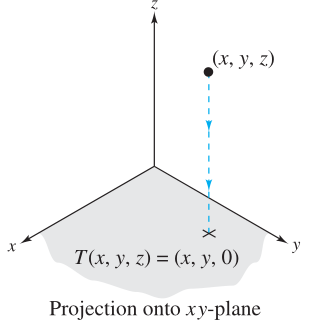
\includegraphics[width = 4cm]{images/proj3d.png}
    \end{minipage}
    \begin{minipage}{0.6\linewidth}
        A linear transformation $T: \R^3 \to \R^3$ represented by
        \[A = \begin{bmatrix}
            1 & 0 & 0\\
            0 & 1 & 0\\
            0 & 0 & 0
        \end{bmatrix}\]
    is called a \textbf{projection} in $\R^3$.

    $T(x,y,z) = (x,y,0)$, in other words, $T$ maps every vector in $\R^3$ to its orthogonal
    projection in the $xy$-plane.
    \end{minipage}

    \textbf{Example 9. \textcolor{blue5}{A Linear Transformation from $M_{m\x n}$ into $M_{n\x m}$}}

    Let $T: M _{m ,n} \to M _{n,m}$ be the function that maps an $m \x n$ matrix $A$ to its transpose.
    \[T(A)   = A^T\]
    Show that $T$ is a linear transformation.

    \textit{ \textcolor{blue5}{SOLUTION.} } Let $A$ and $B$ be  $m \times n$ matrices. Then,
    \begin{equation*}
        \begin{split}
            T(A + B) &= (A + B)^T \\
                     &= A^T + B^T \\
                     &= T(A) + T(B)
        \end{split}
    \end{equation*}

    and
    \begin{equation*}
        \begin{split}
            T(cA) &= (cA)^T \\
                  &= c(A^T) \\
                  &= cT(A)
        \end{split}
    \end{equation*}
    

    \textbf{Example 10. \textcolor{blue5}{The Differential Operator (Calculus)}}

    Let $C'[a,b]$ be the set of all functions whose derivatives are continuous on$[a,b]$. Show that the differential
    operator $D_x$ defines a linear transformation from $C'[a,b]$ into $C[a,b]$.

    \textit{\textcolor{blue9}{SOLUTION.}} Using operator notation, we can write
    \[D_x(f) = \ddfrac{d}{dx} (f) \]
    where $f \in C'[a,b]$. 
    
    \begin{minipage}{0.49\linewidth}
    We have 
    \begin{equation*}
        \begin{split}
            D_x(f + g) = \ddfrac{d}{dx}[f + g] &= \ddfrac{d}{dx}[f] + \ddfrac{d}{dx}[g]\\
                                               &= D_x(f) + D_x(g)
        \end{split}
    \end{equation*}
    \end{minipage} \hfill \vline \hfill
    \begin{minipage}{0.45\linewidth}
    Similarly,
    \begin{equation*}
        \begin{split}
        D_x(cf) = \ddfrac{d}{dx}[cf] &= c \ddfrac{d}{dx}[f] \\
        &= cD_x(f)
        \end{split}
    \end{equation*}    
    \end{minipage}
    
    So, $D_x$ is a linear transformation from $C'[a,b]$ to $C[a,b]$. It's called \textbf{differential operator}.

    For polynomials, the differential operator is $D_x: P_n \to P_{n-1}$ because the derivative of a polynomial function
    of degree $n$ is a polynomial function of degree $n-1$ or less.
    \[D_x( a_nx^n + \cdots + a_1x + a_0 ) = na_nx^{x-1} + \cdots + a_1 \]
    \textbf{Example 11. \textcolor{blue5}{The Definite Integral as a Linear Transformation (Calculus)}}
    
    Let $T: P \to \R$ be defined by
    \[T(p) =  \int_a^b p(x)\,dx\]
    Show that $T$ is a linear transformation from $P$, the vector space of polynomial functions, into $ \R $, the vector space
    of real numbers.

    \textit{\textcolor{blue5}{SOLUTION.}}
    
    Using the properties of definite integrals, we can write

    \begin{minipage}{0.45\linewidth}
    \begin{equation*}
        \begin{split}
            T(p + q) &= \int_a^b [p(x) + q(x)]\,dx \\
                     &= \int_a^b p(x)\,dx + \int_a^b q(x)\,dx \\
                     &= T(p) + T(q)
        \end{split}
    \end{equation*}    
    \end{minipage} \hfill \vline \hfill
    \begin{minipage}{0.50\linewidth}
        and
        \[T(cp) = \int_a^b c[p(x)]\,dx = c\int_a^b p(x)\,dx = cT(p)\]
    \end{minipage}

    So, $T$ is a linear transformation.

    \pagebreak
    \part{The Kernel and Range of a Linear Transformation}
    \begin{tcolorbox}[colback = {blue9}]
         \textbf{Definition of Kernel of a Linear Transformation}

        Let $T: V \to W$ be a linear transformation. Then the set of all vectors \textbf{v} in $V$ that satisfy $T( \textbf{v} ) = \textbf{0} $
        is called the \textbf{kernel} of $T$ and is denoted by $\text{ker}(T)$.
        \[\text{ker}(T) = \{ \textbf{v} \in V : T( \textbf{v} ) = \textbf{0} \} \]
    \end{tcolorbox}
    Sometimes the kernel of a transformation is obvious.

    \textbf{Example 1. \textcolor{blue5}{Finding the Kernel of a Linear Transformation}}

    Let $T: M_{3,2} \to M_{2,3}$ be the linear transformation that maps a $3 \times 2$ matrix $A$ to its transpose.\\
    The kernel of $T$ consists of a single element: the zero matrix in $M_{3,2}$.

    \textbf{Example 2. \textcolor{blue5}{The Kernels of the Zero and Identity Transformations}}\\
    (a) The zero transformation: ker($T$) = $V$.\\
    (b) The identity transformation: ker($T$) = $\{ \textbf{0} \}$.


    \textbf{Example 3. \textcolor{blue5}{Finding the Kernel of a Linear Transformation}}

    Find the kernel of the projection $T: \R^3  \to \R^3 $ represented by
    \[T(x,y,z) = (x,y,0)\]


    \begin{minipage}{0.5\linewidth}
    \textit{\textcolor{blue5}{SOLUTION.}} The kernel consists of all vectors lying on the $z$-axis.
    \[\text{ker}(T) = \{(0,0,z): z \in \R \} \]
    \end{minipage}    \hfill
    \begin{minipage}{0.3\linewidth}
        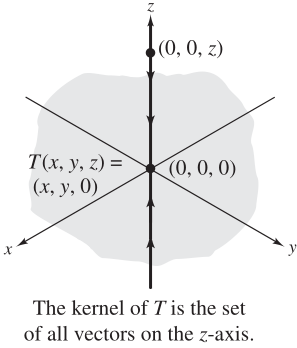
\includegraphics[width = 4cm]{images/zaxis.png}
    \end{minipage}

    These above kernels were fairly easy to find. Generally, the kernel of a linear transformation is not so obvious.

    \textbf{Example 4. \textcolor{blue5}{Finding the Kernel of a Linear Transformation}}

    Find the kernel of the linear transformation $T: \R^2  \to \R^3 $ represented by
    \[T(x_1, x_2) = (x_1 - 2x_2, 0, -x_1)\]

    \textit{\textcolor{blue5}{SOLUTION.}} To find ker($T$), we need to find all $ \textbf{x} = (x_1, x_2)$ in $ \R^2$ such that
    \[T(x_1, x_2) = (x_1 - 2x_2, 0, -x_1) = (0,0,0) \]
    This leads to the homogeneous system
    $\systeme {
        x_1 - 2x_2 = 0,
        0 = 0,
        -x_1 = 0
    }\quad $, which has only the trivial solution.

    So, we have $\text{ker}(T) = \{(0,0)\} = \{ \textbf{0} \}$.

    \textbf{Example 5. \textcolor{blue5}{Finding the Kernel of a Linear Transformation}}

    Find the kernel of the linear transformation $T: \R^3  \to \R^2 $ defined by $T( \textbf{x} ) = A \textbf{x}$, where
    \[A = \begin{bmatrix}
        1 & -1 & -2 \\
        -1 & 2 & 3
    \end{bmatrix}\]
    \textit{\textcolor{blue5}{SOLUTION.}} The kernel of $T$ is the set of all \textbf{x} = $(x_1, x_2, x_3)$ in $ \R^3 $ such that 
    \[T(x_1, x_2, x_3) = (0,0)\]
    From this equation, we can write the homogeneous system
    \[\begin{bmatrix}
        1 & -1 & -2 \\
        -1 & 2 & 3
    \end{bmatrix} \begin{bmatrix}
        x_1 \\ x_2 \\ x_3
    \end{bmatrix} = \begin{bmatrix}
        0 \\ 0 
    \end{bmatrix} 
    \implies \systeme {
        x_1 - x_2 - 2x_3 = 0,
        -x_1 + 2x_2 + 3x_3 = 0
    }\]
    Writing the augmented matrix of this system in reduced row-echelon form produces
    \[ \begin{bmatrix}
        1 & 0 & -1 & 0\\
        0 & 1 & 1 & 0
    \end{bmatrix} \implies
    \begin{cases}{}
        x_1 = x_3 \\
        x_2 = -x_3
    \end{cases}    \]
    Using the parameter $t = x_3$ produces the family of solutions
    \[ \begin{bmatrix}
    x_1 \\ x_2 \\ x_3 
    \end{bmatrix} =  \begin{bmatrix}
        t \\ -t \\ t
    \end{bmatrix} = t\begin{bmatrix}
        1 \\ -1 \\ 1
    \end{bmatrix} \]
    So, the kernel of $T$ is represented by
    \begin{equation*}
        \begin{split}
            \text{ker}(T) &= \{t(1,-1,1): t \in \R \} \\
                          &= \text{span}{(1,-1,1)}
        \end{split}
    \end{equation*}
    \begin{tcolorbox}[colback = {blue9}]
        \textit{THEOREM 6.3} \textbf{The Kernel Is a Subspace of \textit{V}}

        The kernel of a linear transformation $T: V \to W$ is a subspace of the domain $V$.
    \end{tcolorbox}
    \textbf{REMARK.} As a result of Theorem 6.3, the kernel $T$ is sometimes called the \textbf{nullspace} of $T$.

    \textbf{Example 6. \textcolor{blue5}{Finding a Basis for the Kernel}}

    Let $T: \R^5  \to \R^4 $ be defined by $T( \textbf{x} ) = A \textbf{x}$, where \textbf{x} is in $ \R^5 $ and
    \[A = \begin{bmatrix}
        1 & 2 & 0 & 1 & -1\\
        2 & 1 & 3 & 1 & 0 \\
        -1 & 0 & -2 & 0 & 1\\
        0 & 0 & 0 & 2 & 8
    \end{bmatrix}\]
    Find a basis for ker($T$) as a subspace of $ \R^5 $.

    \textit{\textcolor{blue5}{SOLUTION.}} Reduce the augmented matrix $[A \vdots \textbf{0}]$ to echelon form as follows.
    \[ \begin{bmatrix}[ccccc|c]
        1 & 0 & 2 & 0 & -1 & 0 \\
        0 & 1 & -1 & 0 & -2 & 0\\
        0 & 0 & 0 & 1 & 4 & 0 \\
        0 & 0 & 0 & 0 & 0 & 0
    \end{bmatrix} \implies 
    \systeme{
        x_1 = -2x_3 + x_5,
        x_2 = x_3 + 2x_5,
        x_4 = -4x_5
    }\]
    Letting $x_3 = s$ and $x_5 = t$, we have
    \[ \textbf{x} = \begin{bmatrix}
        x_1 \\ x_2 \\ x_3 \\ x_4 \\ x_5
    \end{bmatrix} = \begin{bmatrix}
        -2s + t \\
        s + 2t \\
        s + 0t \\
        0s - 4t \\
        0s +t
    \end{bmatrix} = s \begin{bmatrix}
    -2 \\ 1 \\ 1 \\ 0 \\ 0
    \end{bmatrix} + t \begin{bmatrix}
        1 \\ 2 \\ 0 \\ -4 \\ 1
    \end{bmatrix} \]
    So one basis for the kernel $T$ is $B = \{(-2, 1, 1, 0, 0), (1, 2, 0, -4, 1)\}$.

%    \begin{thm*}{ \textit{COROLLARY TO THEOREM 6.3} }

 %   \end{thm*}    
    
    \begin{Lemma}[\textit{COROLLARY}]
    Let $T: \R^n  \to \R^m $ be the linear transformation given by $T( \textbf{x} ) = A \textbf{x}$. Then the kernel of $T$
    is equal to the solution space of $A \textbf{x} = \textbf{0}$.
    \[ \text{ker}(T) = N(A)\]

    \end{Lemma}

    \section{The Range of a Linear Transformation}
    Two critical subspaces associated with a linear transformation are the \textbf{kernel} and the \textbf{range} of $T$.
    \[ \text{range}(T) = \{T( \textbf{v} ): \textbf{v} \in V \} \]

    \begin{tcolorbox}[colback = {blue9}]
        \textit{THEOREM 6.4} \textbf{The Range of \textit{T} Is a Subspace of \textit{W}}

        The range of a linear transformation $T: V \to W$ is  a subspace of $W$.
    \end{tcolorbox}
    \begin{minipage}{0.25\linewidth}
        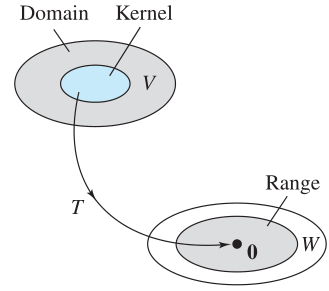
\includegraphics[width = 4cm]{images/fig66.png}
    \end{minipage}
    \begin{minipage}{0.7\linewidth}
        \textbf{Note.} The kernel and range of $T: V \to W$ are subspaces of $V$ and $W$, respectively.
    \end{minipage}

    To find a basis for the \textbf{range} of $T( \textbf{x} ) = A \textbf{x}$, observe that the range consists of 
    all vectors \textbf{b} such that the system $A \textbf{x} = \textbf{b}$ is \textit{consistent}. By writing the system
    \[ \begin{bmatrix}
        a_{11} & a_{12} & \cdots & a_{1n} \\
        a_{21} & a_{22} & \cdots & a_{2n} \\
        \vdots & \vdots & & \vdots \\
        a_{m1} & a_{m2} & \cdots & a_{mn}
    \end{bmatrix}
    \begin{bmatrix}
        x_1 \\
        x_2\\
        \vdots \\
        x_n
    \end{bmatrix}  = 
    \begin{bmatrix}
        b_1 \\
        b_2\\
        \vdots \\
        b_m
    \end{bmatrix} \]
    in the form 
    \[ A \textbf{x} = x_1 \begin{bmatrix}
        a_{11} \\
        a_{21} \\
        \vdots \\
        a_{m1}
    \end{bmatrix} + x_2 \begin{bmatrix}
    a_{12} \\
    a_{22} \\
    \vdots \\
    a_{m2}
\end{bmatrix} + \cdots + x_n \begin{bmatrix}
a_{1n} \\
a_{2n} \\
\vdots \\
a_{mn}
\end{bmatrix} = \begin{bmatrix}
b_1 \\
b_2\\
\vdots \\
b_n
\end{bmatrix}  = \textbf{b}\]
   You can see that \textbf{b} is in the range of $T$ if and only if \textbf{b} is a linear combination of the column vectors
   of $A$. So \textit{the column space of $A$ is the same as the range of $T$.}
    \begin{Lemma}[ \textit{COROLLARY} ]
        Let $T: \R^n  \to \R^m $ to be the linear transformation given by $T( \textbf{x}  = A \textbf{x}$.) Then the column
        space of $A$ is equal to the range of $T$.
        \[R(A) = \text{range}(T)\]
    \end{Lemma}
    \textbf{Example 7. \textcolor{blue5}{Finding a Basis for the Range of a Linear Transformation}}

    For the linear transformation $ \R^5  \to \R^4 $ from the Example 6, find a basis for the range of $T$.

    \textit{\textcolor{blue5}{SOLUTION.}} The echelon from of $A$ was calculated in Example 6.
        \[A =
        \begin{bmatrix}[rrrrr]
        1 & 2 & 0 & 1 & -1\\
        2 & 1 & 3 & 1 & 0 \\
        -1 & 0 & -2 & 0 & 1\\
        0 & 0 & 0 & 2 & 8
    \end{bmatrix} \implies 
            \begin{bmatrix}[rrrrr]
        1 & 0 & 2 & 0 & -1  \\
        0 & 1 & -1 & 0 & -2  \\
        0 & 0 & 0 & 1 & 4  \\
        0 & 0 & 0 & 0 & 0 
    \end{bmatrix} \]
    Because the leading 1's appear in columns 1, 2, and 4 of the reduced matrix on the right, the corresponding 
    column vectors of $A$ form a basis for $R(A)$. One basis for range($T$) is
    \[ B = \{ (1,2,-1,0), (2,1,0,0), (1,1,0,2)\} \]
    \begin{tcolorbox}[colback = {blue9}]
        \textbf{Definition of Rank and Nullity of a Linear Transformation}

        Let $T: V \to W$ be a linear transformation. The dimension of the kernel of $T$ is called the \textbf{nullity} of $T$.
        The dimension of the range of $T$ is called the \textbf{rank} of $T$.
        \[ \textbf{nullity}(T) = \text{dim}(\text{ker}(T)) \]
        \[ \textbf{rank}(T) = \text{dim}(\text{range}(T)) \]
    \end{tcolorbox}
    \textbf{REMARK.} If $T$ is provided by a matrix $A$, then rank($T$) = rank($A$).
    \begin{tcolorbox}[colback = {blue9}]
        \textit{THEOREM 6.5} \textbf{Sum of Rank and Nullity}

        Let $T: V \to W$ be a linear transformation from an $n$-dimensional vector space $V$ into a vector space $W$. Then the sum
        of the dimensions of the range and the kernel is equal to the dimension of the \textbf{domain}.
        \[ \text{rank}(T) + \text{nullity}(T) = n \]
        \[\text{dim(range)}] + \text{dim(kernel)} = \text{dim(domain)} \]
    \end{tcolorbox}

    \section{One-to-One and Onto Linear Transformation}

    \begin{minipage}{0.61\linewidth}
            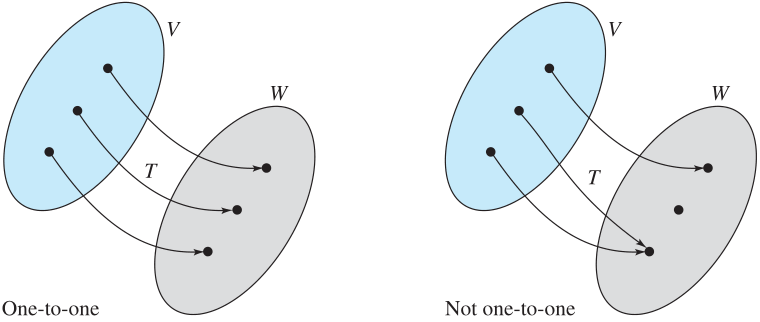
\includegraphics[width = 10cm]{images/1to1.png}    
    \end{minipage} \hfill
    \begin{minipage}{0.36\linewidth}
        A function $T: V \to W$ is called \textbf{one-to-one} if the preimage of every \textbf{w} in the range consists of a single
        vector.
        \[ T( \textbf{u} ) = T( \textbf{v} ) \implies \textbf{u} = \textbf{v} \]
        for all \textbf{u} and \textbf{v} in $V$.
    \end{minipage}
    \begin{tcolorbox}[colback = {blue9}]
        \textit{THEOREM 6.6} \textbf{One-to-One Linear Transformations}

        Let $T: V \to W$ be a linear transformation. Then $T$ is one-to-one if and only if ker($T$) = \{\textbf{0}\}.
    \end{tcolorbox}

    A function $T: V\to W$ is called \textbf{onto} if every element in $W$ has a preimage in $V$. In other words, $T$ is 
    onto $W$ when $W$ is equal to the range of $T$.
    \begin{tcolorbox}[colback = {blue9}]
        \textit{THEOREM 6.7} \textbf{Onto Linear Transformations}

        Let $T: V\to W$ be a linear transformation, where $W$ is finite dimensional. Then $T$ is onto $W$ if and only if
        the rank of $T$ is equal to the dimension of $W$.
    \end{tcolorbox}

    For vector spaces of equal dimensions, you can combine the results of Theorems 6.5, 6.6 and 6.7 to obtain
    the next theorem relating to the concepts of one-to-one and onto.
    \begin{tcolorbox}[colback = {blue9}]
        \textit{THEOREM 6.8} \textbf{One-to-One and Onto Linear Transformations}

        Let $T: V \to W$ be a linear transformation with vector spaces $V$ and $W$ \textit{both} of dimension $n$.
        Then $T$ is one-to-one if and only if it is onto.
    \end{tcolorbox}
    \textbf{Example 11. \textcolor{blue5}{Summarizing Several Results}}

    The linear transformation $T: \R^n  \to \R^m $ is represented by $T( \textbf{x} ) = A \textbf{x}$. Find the nullity
    and rank of $T$, then determine whether $T$ is one-to-one, onto, or neither.
    \begin{equation*}
        \begin{array}{ll}
           \text{(a)} A = \begin{bmatrix}
            1 & 2 & 0 \\
            0 & 1 & 1 \\
            0 & 0 & 1
        \end{bmatrix} & 
        \text{(b)} A = \begin{bmatrix}
            1 & 2 \\
            0 & 1 \\
            0 & 0
        \end{bmatrix} \\

        \text{(c)} A = \begin{bmatrix}
            1 & 2 & 0 \\
            0 & 1 & -1
        \end{bmatrix} & 
        \text{(d)} A = \begin{bmatrix}
            1 & 2 & 0 \\
            0 & 1 & 1 \\
            0 & 0 & 0
        \end{bmatrix}
        \end{array}
    \end{equation*}

    \begin{center}
                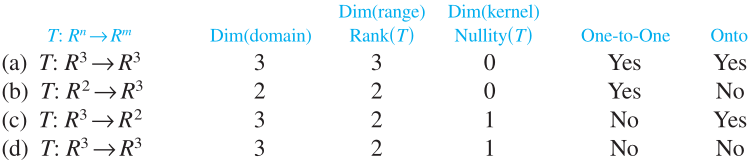
\includegraphics[width = 12cm]{images/4typeeg11.png}
    \end{center}

    \section{Isomorphisms of Vector Spaces}
    This is a very important concept that can be a great aid in your understanding of vector spaces. The concept
    provides a way to think of distinct vector spaces as being "essentially the same" - at least with respect to
    the operations of vector addition and scalar multiplication.
    \begin{Def}[Isomorphism]
        A linear transformation $T: V \to W$ that is one-to-one and onto are called an \textbf{isomorphism}.

        If $V$ and $W$ are vector spaces such that there exists an isomorphism from $V$ to $W$, then $V$ and $W$
        are \textbf{isomorphic} to each other.
    \end{Def}

    \begin{tcolorbox}[colback = {blue9}]
        \textit{THEOREM 6.9} \textbf{Isomorphic Spaces and Dimension}

        Two finite-dimensional vector spaces $V$ and $W$ are isomorphic if and only if they are of the same
        dimension.
    \end{tcolorbox}

    \textbf{Example 12. \textcolor{blue5}{Isomorphic Vector Spaces}}

    The vectors listed below are mutually isomorphic.\\
    (a) $ \R^4 = 4$-space\\
    (b) $M_{4,1} =$ space of all $4 \times 1$ matrices \\
    (c) $M_{2,2} =$ space of all $2 \times 2$ matrices\\
    (d) $P_3 =$ space of all polynomials of degree 3 or less\\
    (e) $V = \{(x_1, x_2, x_3, x_4, 0): x_i \in \R  \}\quad$(subspace of $ \R^5 $)
    \pagebreak
    \part{Matrices for Linear Transformations}
    \begin{minipage}{0.6\linewidth}
    Which representation of $T \R^3  \to \R^3 $ is better,
    \[T(x_1, x_2, x_3) = (2x_1 + x_2 -x_3, -x_1 + 3x_2 -2x_3, 3x_2 + 4x_3)\]
    or 
    \[T( \textbf{x} ) = A \textbf{x} = \begin{bmatrix}
        2 & 1 & -1 \\
        -1 & 3 & -2\\
        0 & 3 & 4
    \end{bmatrix} \begin{bmatrix}
    x_1 \\
    x_2\\
    x_3
    \end{bmatrix} ?\] 
    \end{minipage}
    \begin{minipage}{0.38\linewidth}
    \begin{Ans}
        The second one is better for 3 reasons: it is simpler to write, simpler to read, and more easily adapted
        for computer use.
    \end{Ans}     
    \end{minipage}

    The key to representing $T: V \to W$ by a matrix is to determine how it acts on a \textbf{basis} of $V$. Once you know the
    image of every vector in the basis, you can determine $T( \textbf{v} )$ for any \textbf{v} $\in V$.
    \begin{tcolorbox}[colback = {blue9}]
        \textit{THEOREM 6.10} \textbf{Standard Matrix for a Linear Transformation}

        Let $T: \R^n  \to \R^m $ be a linear transformation such that
        \[ T( \textbf{e}_1 ) = \begin{bmatrix}
            a_{11} \\
            a_{21} \\
            \vdots \\
            a_{m1}
        \end{bmatrix} , 
        T( \textbf{e}_2 ) = \begin{bmatrix}
            a_{12} \\
            a_{22} \\
            \vdots \\
            a_{m2}
        \end{bmatrix}, \dots, 
        T( \textbf{e}_n ) = \begin{bmatrix}
            a_{1n} \\
            a_{2n} \\
            \vdots \\
            a_{mn}
        \end{bmatrix} \]
        Then the $m \times n$ matrix whose $n$ columns correspond to $T( \textbf{e}_i )$,
        \[ A = \begin{bmatrix}
            a_{11} & a_{12} & \cdots & a_{1n} \\
            a_{21} & a_{22} & \cdots & a_{2n} \\
            \vdots & \vdots & & \vdots \\
            a_{m1} & a_{m 2} & \cdots & a_{m n}
        \end{bmatrix} \]
        is such that $T( \textbf{v}) = A \textbf{v}$ for every \textbf{v} in $ \R^n $. A is called the \textbf{standard matrix} for $T$.
    \end{tcolorbox}

    \textbf{Example 1. \textcolor{blue5}{Finding the Standard Matrix for a Linear Transformation}}

    Find the standard matrix for $T: \R^3  \to \R^2 $ defined by
    \[T(x,y,z) = (x - 2y, 2x + y)\]
    \textit{\textcolor{blue5}{SOLUTION.}} Begin by finding the images of $ \textbf{e}_1, \textbf{e}_2$ and $ \textbf{e}_3$.
    \begin{center}
        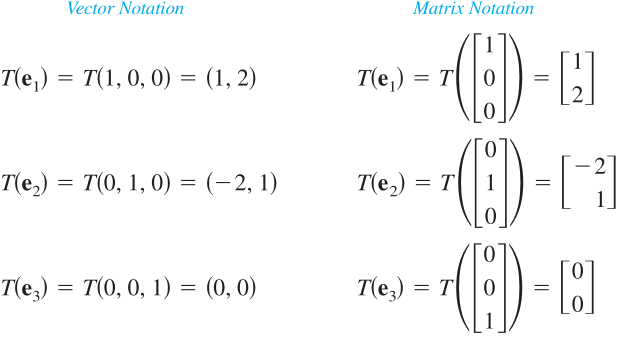
\includegraphics[width = 9.5cm]{images/eg1standardmatrix.png}
    \end{center}
    By Theorem 6.10, we have
    \[ A = [T(\textbf{e}_1) \vdots T( \textbf{e}_2 ) \vdots T( \textbf{e}_3 )] = 
        \begin{bmatrix}
            1 & -2 & 0 \\
            2 & 1 & 0
        \end{bmatrix} \]
    \textbf{Example 2. \textcolor{blue5}{Finding the Standard Matrix for a Linear Transformation}}

    \begin{minipage}{0.3\linewidth}
        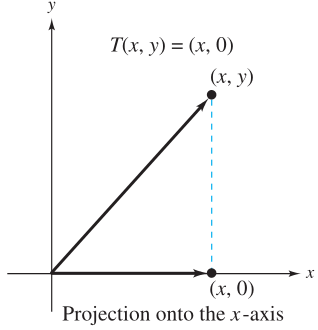
\includegraphics[width = 4.5cm]{images/xproj.png}
    \end{minipage}
    \begin{minipage}{0.65\linewidth}
    The linear transformation $T: \R^2  \to \R^2 $ is given by projecting each point in $ \R^2 $ onto the $x$-axis.
    \[T(x,y) = T(x,0)\]
    The standard matrix for $T$ is
    \begin{equation*}
        \begin{split}
            A &= \begin{bmatrix}
                T(1,0) & \vdots & T(0,1)
            \end{bmatrix} = \begin{bmatrix}
                  1 & 0\\
                  0 & 0
              \end{bmatrix}
        \end{split}
    \end{equation*}
    \end{minipage}

    \section{Composition of Linear Transformations}

    \begin{minipage}{0.6\linewidth}
    The \textbf{composition} , $T$, of $T_1: \R^n  \to \R^m $ with $T_2: \R^m  to \R^p$ is defined by
    \[T( \textbf{v} ) = T_2(T_1( \textbf{v} )) \]    
    where \textbf{v} is a vector $ \R^n $. This composition is denoted by
    \[T = T_2 \circ T_1\]
    \end{minipage} \hfill
    \begin{minipage}{0.3\linewidth}
        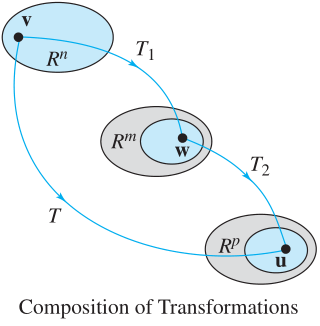
\includegraphics[width = 4cm]{images/compos.png}
    \end{minipage}
    \begin{tcolorbox}[colback = {blue9}]
        \textit{THEOREM 6.11} \textbf{Composition of Linear Transformations}

        Let $T_1: \R^n  \to \R^m $ and $T_2: \R^m  \to \R^p$ be linear transformation with standard matrices $A_1$ and $A_2$.

        The \textbf{composition} $T: \R^n  \to \R^p$, defined by $T( \textbf{v}) = T_2(T_1( \textbf{v} ))$, is a linear transformation,
        which standard matrix $A$ is given by
        \[A = A_2A_1\]
    \end{tcolorbox}
    \textbf{REMARK.} Theorem 6.11 can be generalized to cover the composition of $n$ linear transformation. That is,
    if the standard matrices of     $T_1, T_2, \dots, T_n$ are $A_1, A_2, \dots, A_n$, then 
    \[A = A_nA_{n-1}\cdots A_2A_1\]
    \textbf{Example 3. \textcolor{blue5}{The Standard Matrix for a Composition}}

    Let $T_1$ and $T_2$ be linear transformations from $ \R^3 $ to $ \R^3 $ such that
    \[T_1(x,y,z) = (2x + y, 0 , x+z) \quad \text{ and  } \quad T_2(x,y,z) = (x - y, z, y)\]
    Find the standard matrices for the compositions $T = T_2 \circ T_1$ and $T' = T_1 \circ T_2$.

    \textit{\textcolor{blue5}{SOLUTION.}} The standard matrices for $T_1$ and $T_2$ are
    \[A_1 = \begin{bmatrix}
        2 & 1 & 0 \\
        0 & 0 & 0\\
        1 & 0 & 1
    \end{bmatrix} \quad 
    \text{and} \quad
    A_2 = \begin{bmatrix}
        1 & -1 & 0 \\
        0 & 0 & 1 \\
        0 & 1 & 0
    \end{bmatrix}\]
    By Theorem 6.11, the standard matrix for $T$ is
    \[A = A_2A_1 = \begin{bmatrix}
        1 & -1 & 0 \\
        0 & 0 & 1 \\
        0 & 1 & 0
    \end{bmatrix} \begin{bmatrix}
        2 & 1 & 0 \\
        0 & 0 & 0\\
        1 & 0 & 1
    \end{bmatrix} = \begin{bmatrix}
        2 & 1 & 0 \\
        1 & 0 & 1 \\
        0 & 0 & 0
    \end{bmatrix} \]
    and the standard matrix for $T'$ is
    \[A' = A_1A_2 = \begin{bmatrix}
        2 & 1 & 0 \\
        0 & 0 & 0\\
        1 & 0 & 1
    \end{bmatrix} \begin{bmatrix}
        1 & -1 & 0 \\
        0 & 0 & 1 \\
        0 & 1 & 0
    \end{bmatrix} = \begin{bmatrix}
        2 & -2 & 1 \\
        0 & 0 & 0\\
        1 & 0 & 0
    \end{bmatrix}\]
    
    Another benefit of matrix representation is that it can represent the \textbf{inverse} of a linear transformation.
    \begin{Def}[Inverse of Linear Transformation]
        If $T_1: \R^n  \to \R^n $ and $T_2: \R^n  \to \R^n $ are linear transformations such that for every \textbf{v} $\in \R^n $
        \[T_2(T_1( \textbf{v} )) = \textbf{v} \quad \text{and} \quad T_1(T_2( \textbf{v} )) = \textbf{v},\]
        then $T_2$ is called the \textbf{inverse} of $T_1$, and $T_1$ is said to be \textbf{invertible}.
    \end{Def}
    If $T_1$ is invertible, the inverse is \textbf{unique} and is denoted by $T_1^{-1}$. The inverse of $T$ can be thought as
    \textit{undoing the mapping} done by $T$ - in other words, mapping back to the preimage under $T$.
    \begin{tcolorbox}[colback = {blue9}]
        \textit{THEOREM 6.12} \textbf{Existence of an Inverse Transformation}

        Let $T: \R^n \to \R^n $ be a linear transformation with standard matrix $A$. Then the following conditions are
        equivalent.
        
        1. $T$ is invertible.
        
        2. $T$ is an isomorphism.
        
        3. $A$ is invertible.

        And, the standard matrix for $T^{-1}$ is $A^{-1}$.
    \end{tcolorbox}
    %section 4.6 for more information
    \section{Nonstandard Bases and General Vector Spaces}
    We will now consider the problem of finding a matrix for $T: V \to W$, where $B$ and $B'$ are ordered bases for $V$ and $W$.
    In order to represent $T$, $A$ must be multipled by a \textit{coordinate matrix relative to $B$}. The result will be a 
    \textit{coordinate matrix relative to $B'$}. That is,
    \[[T( \textbf{v} )]_{B'} = A[ \textbf{v} ]_B\]
    $A$ is called the \textbf{matrix of $T$ relative to the bases $B$ and $B'$}.
    \begin{tcolorbox}[colback = {blue9}]
        \textbf{Transformation Matrix for Nonstandard Bases.}

        Let $V$ and $W$ be finite-dimensional vector spaces with bases $B$ and $B'$, where
        \[B = \{ \textbf{v}_1, \textbf{v}_2, \dots, \textbf{v}_n\}\]
        If $T: V \to W$ is a linear transformation such that
        \[ [T( \textbf{v}_1 )]_{B'} = \begin{bmatrix}
            a_{11} \\
            a_{21} \\
            \vdots \\
            a_{m1}
        \end{bmatrix} ,
        [T( \textbf{v}_2 )]_{B'} = \begin{bmatrix}
            a_{12} \\
            a_{22} \\
            \vdots \\
            a_{m2}
        \end{bmatrix}, \dots,
        [T( \textbf{v}_n )]_{B'} = \begin{bmatrix}
            a_{1n} \\
            a_{2n} \\
            \vdots \\
            a_{mn}
        \end{bmatrix} \]
        then the $m \times n$ matrix whose $n$ columns correspond to $[T( \textbf{v}_i )]_{B'}$
        \[A = \begin{bmatrix}
            a_{11} & a_{12} & \cdots & a_{1n} \\
            a_{21} & a_{22} & \cdots & a_{2n} \\
            \vdots & \vdots & & \vdots \\
            a_{m1} & a_{m 2} & \cdots & a_{m n}
        \end{bmatrix} \]
        is such that $[T( \textbf{v} )]_{B'} = A[ \textbf{v} ]_B$ for $\forall \textbf{v} \in V$.
    \end{tcolorbox}
    \textbf{Example 5. \textcolor{blue5}{Finding a Matrix Relative to Nonstandard Matrix}}

    Let $T: \R^2 \to \R^2 $ be a linear transformation defined by 
    \[T(x_1,x_2) = (x_1 + x_2, 2x_1 - x_2) \]
    Find the matrix for $T$ relative to the bases
    \[B = \{ \overset{ \textbf{v}_1 }{(1,2)}, \overset{ \textbf{v}_2 }{(-1,1)} \} \quad \text{and} \quad
        B' = \{ \overset{ \textbf{w}_1 }{(1,0)}, \overset{ \textbf{w}_2 }{(0,1)} \}\]
    \textit{\textcolor{blue5}{SOLUTION.}} By the definition of $T$, we have
    \begin{equation*}
        \begin{split}
            T( \textbf{v}_1 ) &= T(1,2) = (3,0) = 3\textbf{w}_1 + 0 \textbf{w}_2 \\
            T( \textbf{v}_2 ) &= T(-1,1) = (0,-3) = 0 \textbf{w}_1 - 3 \textbf{w}_2
        \end{split}
    \end{equation*}
    The coordinate matrices for $T( \textbf{v}_1 )$ and $T( \textbf{v}_2 )$ relative to $B'$ are
   \[[T( \textbf{v}_1 )]_{B'}  = \begin{bmatrix}
       3 \\ 0
   \end{bmatrix}  \quad \text{and} \quad 
   [T( \textbf{v}_2 )]_{B'}  = \begin{bmatrix}
       0 \\ -3
   \end{bmatrix}\]
   The matrix for $T$ relative to $B$ and $B'$ is $A = \begin{bmatrix}[rr]
       3 & 0 \\ 0 & -3
   \end{bmatrix}$.

   \textbf{Example 6. \textcolor{blue5}{Using a Matrix to Represent a Linear Transformation}}

   Using $T: \R^2  \to \R^2 $ from Example 5, find $T( \textbf{v} ) $, where $ \textbf{v} = (2,1)$.

   \textit{\textcolor{blue5}{SOLUTION.}} Using the basis $B$, we find $[ \textbf{v} ]_B = \begin{bmatrix}
       1 \\ -1
   \end{bmatrix}$. So,$[T( \textbf{v} )]_{B'} = A[ \textbf{v} ]_B = 
   \begin{bmatrix}
       3 & 0 \\ 0 & -3
   \end{bmatrix} \begin{bmatrix}
       1 \\ -1
   \end{bmatrix} = \begin{bmatrix}
       3 \\ 3
   \end{bmatrix}$.\\
   It follows that $T( \textbf{v} ) = 3(1,0) + 3(0,1) = (3,3)$.

   In the special case, where $V = W$ and $B = B'$, then $A$ is called the \textbf{matrix of $T$ relative to basis $B$}. The matrix
   of the identity transformation is just $I_n$.

   \textbf{Example 7. \textcolor{blue5}{A Matrix for the Differential Operator (Calculus)}}

   Let $D_x: P_2 \to P_1$ be the differential operator that maps a quadratic polynomial $p$ onto its derivative $p'$.
   Find the matrix for $D_x$ using the bases
   \[B = \{1, x, x^2\} \quad \text{and} \quad B' = \{1, x \}\]

   \textit{\textcolor{blue5}{SOLUTION.}} The derivatives of the basis vectors are
   \begin{equation*}
       \begin{split}
           D_x(1) &= 0 = 0(1) + 0(x) \\
           D_x(x) &= 1 = 1(1) + 0(x) \\
           D_x(x^2) &= 2x = 0(1) + 2(x)
       \end{split}
   \end{equation*}
   So, the matrix for $D_x$ is $A = \begin{bmatrix}
       0 & 1 & 0 \\
       0 & 0 & 2
   \end{bmatrix}$. Note that this matrix \textit{does} produce the derivative of a quadratic polynomial $p(x) = a + bx + cx^2$.
   \[Ap = \begin{bmatrix}
       0 & 1 & 0 \\
       0 & 0 & 2
   \end{bmatrix} \begin{bmatrix}
       a \\ b \\ c
   \end{bmatrix} = \begin{bmatrix}
       b \\ 2c
   \end{bmatrix} \]
    \pagebreak
   \part{Transition Matrices and Similarity}
   The matrix for $T: V \to V$ depends on the \textit{basis} of $V$. In other words, the matrix for $T$ relative to a basis $B$ is different
   from the one for $B'$.

   \begin{Ques}
       Is it possible to find a basis $B$ such that the matrix for $T$ relative to $B$ is diagonal? The solution will be discussed 
       in Chapter 7. We will see how matrices for $T$ relative to 2 different bases are related.
   \end{Ques}
    In this section, $A, A', P$ and $P^{-1}$ represent the 4 square matrices listed below.

    \begin{minipage}{0.38\linewidth}
    1. Matrix for $T$ relative to $B$:    \\
    2. Matrix for $T$ relative to $B'$:     \\
    3. Transition matrix from $B'$ to $B$:   \\
    4. Transition matrix from $B$ to $B'$:    
    \end{minipage}
    \begin{minipage}{0.3\linewidth}
        $A$\\
        $A'$\\
        $P$\\
        $P^{-1}$
    \end{minipage}

    {\color{blue9} \rule{10.5cm}{0.3mm}}

    There are 2 ways to get from the coordinate matrix $[ \textbf{v} ]_{B'}$ to  $[T( \textbf{v} )]_{B'}$.

    \begin{minipage}{0.44\linewidth}
        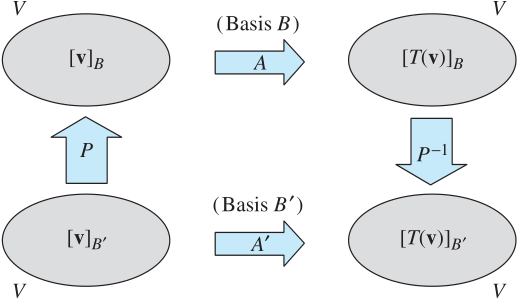
\includegraphics[width = 7cm]{images/transition.png}
    \end{minipage}
    \begin{minipage}{0.53\linewidth}
    One way is direct, using $A'$ to obtain: \[ A'[ \textbf{v} ]_{B'} = [T( \textbf{v} )]_{B'} \]
    The other way is indirect, using $P, A$ and $P^{-1}$ to obtain
    \[P^{-1}AP[ \textbf{v} ]_{B'} = [T( \textbf{v} )]_{B'}\]
    \end{minipage}
    
    \begin{Conc}
        By the definition of the matrix of a linear transformation relative to a basis, this implies that
        \[A' = P^{-1}AP\]
    \end{Conc}

    \textbf{Example 1. \textcolor{blue5}{Finding a Matrix of a Linear Transformation}}

    Find the matrix $A$ for $T: \R^2  \to \R^2 $
    \[T(x_1, x_2) = (2x_1 - 2x_2, -x_1 + 3x_2)\]

    \textit{\textcolor{blue5}{SOLUTION.}} The standard matrix for $T$ is $A = \begin{bmatrix}
        2 & -2 \\
        -1 & 3
    \end{bmatrix}$.

    The transition matrix from $B'$ to $B$ is $P = \begin{bmatrix}
        1 & 1 \\
        0 & 1
    \end{bmatrix}$.
    
    The inverse of this matrix is the transition matrix from $B$ to $B'$: $P^{-1} = \begin{bmatrix}
        1 & -1 \\
        0 & 1
    \end{bmatrix}$.

    The matrix for $T$ relative to $B'$ is \[A' = P^{-1}AP = \begin{bmatrix}
        1 & -1 \\ 0 & 1
    \end{bmatrix} \begin{bmatrix}
        2 & -2 \\ -1 & 3
    \end{bmatrix} \begin{bmatrix}
        1 & 1 \\ 0 & 1
    \end{bmatrix} = \begin{bmatrix}
        3 & -2\\
        -1 & 2
    \end{bmatrix}\]

    \textbf{Example 2. \textcolor{blue5}{Finding a Matrix for a Linear Transformation}}

    Let 
    \[B = \{(-3, 2), (4, -2)\} \quad \text{and} \quad B' = \{(-1,2), (2,-2) \}\]
    be bases for $ \R^2 $, and let 
    \[A = \begin{bmatrix}[rr]
        -2 & 7 \\
        -3 & 7
    \end{bmatrix}\]
    be the matrix for $T: \R^2  \to  \R^2 $ relative to $B$. Find $A'$, the matrix of $T$ relative to $B'$.

    \textit{\textcolor{blue5}{SOLUTION.}} We can easily obtain 
    \[P = \begin{bmatrix}[rr]
        3 & -2 \\
        2 & -1
    \end{bmatrix} \quad \text{and} \quad 
    P^{-1} = \begin{bmatrix}[rr]
        -1 & 2 \\
        -2 & 3
    \end{bmatrix}\]
    So the matrix of $T$ relative to $B'$ is 
    \[A' = P^{-1}AP = 
        \begin{bmatrix}[rr]
        -1 & 2 \\
        -2 & 3
    \end{bmatrix}
    \begin{bmatrix}[rr]
        -2 & 7 \\
        -3 & 7
    \end{bmatrix}
        \begin{bmatrix}[rr]
        3 & -2 \\
        2 & -1
    \end{bmatrix} = \begin{bmatrix}
        2 & 1 \\
        -1 & 3
    \end{bmatrix} \]
    \textbf{REMARK.} It is instructive to note that $T$ in Example 2 is represented by the rule
    $T(x,y) = (x - \frac{3}{2}y, 2x + 4y)$.

    \section{Similar Matrices}
    \begin{Def}[Similar Matrices]
        For square matrices $A$ and $A'$ of order $n$, $A'$ is said to be \textbf{similar} to $A$ if there exist an invertible
        matrix $P$ such that $A' = P^{-1}AP$.
    \end{Def}
    If $A'$ is similar to $A$, then it is also true that $A$ is similar to $A'$. Just simply say that \textbf{\textit{A} and \textit{A'} are similar}.
    \begin{tcolorbox}[colback = {blue9}]
        \textit{THEOREM 6.13} \textbf{Properties of Similar Matrices}

        Let $A,B$ and $C$ be square matrices of order $n$. Then the following properties are true. \\
        1. $A$ is similar to $A$.\\
        2. If $A$ is similar to $B$, then $B$ is similar to $A$.\\
        3. If $A$ is similar to $B$ and $B$ is similar to $C$, then $A$ is similar to $C$.
    \end{tcolorbox}
    It follows that any 2 matrices that represent the same $T: V \to  V$ with respect to different bases must be
    similar.

    \textbf{Example 4. \textcolor{blue5}{Similar Matrices}}

    From Example 1, the matrices
    $A = \begin{bmatrix}
        2 & -2 \\
        -1 & 3
    \end{bmatrix} \quad \text{and} \quad
    A' = \begin{bmatrix}
        3 & -2\\
        -1 & 2
    \end{bmatrix} $
    are similar because $A' = P^{-1}AP$, where $P = \begin{bmatrix}
        1 & 1 \\
        0 & 1
    \end{bmatrix}$.

    {\color{blue9} \rule{7cm}{0.3mm}}

    You have seen that the matrix for $T: V \to  V$ depends on the basis used for $V$. 

    What choice of basis will make the matrix for $T$ as \textit{simple} as possible? Is it always
    the \textit{standard} basis? Not necessarily, as the next example will demonstrate.\\
    \textbf{Example 5. \textcolor{blue5}{A Comparision of Two Matrices for a Linear Transformation}}

    Suppose \[A = \begin{bmatrix}
        1 & 3 & 0 \\
        3 & 1 & 0 \\
        0 & 0 & -2
    \end{bmatrix}\]
    is the matrix for $T: \R^3  \to   \R^3 $ relative to the standard basis. Find the matrix for $T$
    relative to the basis
    \[B' = \{(1,1,0), (1,-1,0), (0,0,1)\}\]
    \textit{\textcolor{blue5}{SOLUTION.}} We have 
    \[P = \begin{bmatrix}
        1 & 1 & 0 \\
        1 & -1 & 0 \\
        0 & 0 & 1
    \end{bmatrix} \quad \text{and} \quad 
    P^{-1} = \begin{bmatrix}
        \frac{1}{2} & \frac{1}{2} & 0 \\
        \frac{1}{2} & - \frac{1}{2} & 0\\
        0 & 0 & 1
    \end{bmatrix}\]
    So, the matrix for $T$ relative to $B'$ is 
    \begin{equation*}
        \begin{split}
            A' &= P^{-1}AP \\
               &= \begin{bmatrix}
        \frac{1}{2} & \frac{1}{2} & 0 \\
        \frac{1}{2} & - \frac{1}{2} & 0\\
        0 & 0 & 1
    \end{bmatrix}\begin{bmatrix}
        1 & 3 & 0 \\
        3 & 1 & 0 \\
        0 & 0 & -2
    \end{bmatrix}\begin{bmatrix}
        \frac{1}{2} & \frac{1}{2} & 0 \\
        \frac{1}{2} & - \frac{1}{2} & 0\\
        0 & 0 & 1
    \end{bmatrix} \\
               &= \begin{bmatrix}
                   4 & 0 & 0\\
                   0 & -2 & 0\\
                   0 & 0 & -2
               \end{bmatrix}
        \end{split}
    \end{equation*}
    Note that $A'$ is diagonal.

    \section*{ \textcolor{blue5}{Diagonal Matrices} }

    Diagonal matrices have many computational advantages over nondiagonal ones. For instance, for the diagonal
    matrix 
    \[D = \begin{bmatrix}
        d_1 & 0 & \cdots & 0 \\
        0 & d_2 & \cdots & 0\\
        \vdots & \vdots & & \vdots \\
        0 & 0 & \cdots & d_n
    \end{bmatrix}\]
    the $k$th power is represented as follows.
    \[D^k = \begin{bmatrix}
        d_1^k & 0 & \cdots & 0 \\
        0 & d_2^k & \cdots & 0\\
        \vdots & \vdots & & \vdots \\
        0 & 0 & \cdots & d_n^k
    \end{bmatrix}\]
                A diagonal matrix is its own \textit{transpose}. Moreover, if all the diagonal elements are nonzero, then the inverse
    of a diagonal matrix is the matrix whose main diagonal elements are reciprocals of corresponding elements in the
    original one.
        

    \begin{Conc}

    With such computational advantages, it's important to find ways (if possible) to choose a basis for $V$
    such that the transformation matrix is diagonal.

    \end{Conc}
    \pagebreak

    \part{Applications of Linear Transformations}

    \section{The Geometry of Linear Transformations in the Plane}
    
    \begin{Def}[Elementary Matrices for Linear Transformations in the Plane]
        \begin{equation*}
            \begin{array}{ccccc}
                \overset{ \textcolor{blue3}{\textit{Reflection in $y$-Axis}} }{
                    A = \begin{bmatrix}
                        -1 & 0 \\
                        0 & 1
                    \end{bmatrix}
                }
                & \quad &                 \overset{ \textcolor{blue3}{\textit{Reflection in $x$-Axis}} }{
                    A = \begin{bmatrix}
                        1 & 0 \\
                        0 & -1
                    \end{bmatrix}
                }
 & \quad &                 \overset{ \textcolor{blue3}{\textit{Reflection in Line $y = x$}} }{
                    A = \begin{bmatrix}
                        0 & 1 \\
                        1 & 0
                    \end{bmatrix}
                }
 \\
                                \overset{ 
                                    \begin{subarray}{l}
                                         \textcolor{blue3}{\textit{Horizontal Expansion ($k>1$) }}\\
                                    \textcolor{blue3}{\textit{or Contraction ($0<k<1$)} }
                                    \end{subarray}
                                   }{
                    A = \begin{bmatrix}
                        k & 0 \\
                        0 & 1
                    \end{bmatrix}
                }
 & \quad &                 \overset{\begin{subarray}{c}
                                         \textcolor{blue3}{\textit{Vertical Expansion ($k>1$) }}\\
                                    \textcolor{blue3}{\textit{or Contraction ($0<k<1$)} }
                                    \end{subarray}
}{
                    A = \begin{bmatrix}
                        1 & 0 \\
                        0 & k
                    \end{bmatrix}
                }
\\
                                \overset{ \textcolor{blue3}{\textit{Horizontal Shear}} }{
                    A = \begin{bmatrix}
                        1 & k \\
                        0 & 1
                    \end{bmatrix}
                }
 & \quad &                                 \overset{ \textcolor{blue3}{\textit{Vertical Shear}} }{
                    A = \begin{bmatrix}
                        1 & 0 \\
                        k & 1
                    \end{bmatrix}
                }

 & \quad & 
            \end{array}
        \end{equation*}
    \end{Def}

    \textbf{Example 1. \textcolor{blue5}{Reflections in the Plane}}
    \begin{center}
        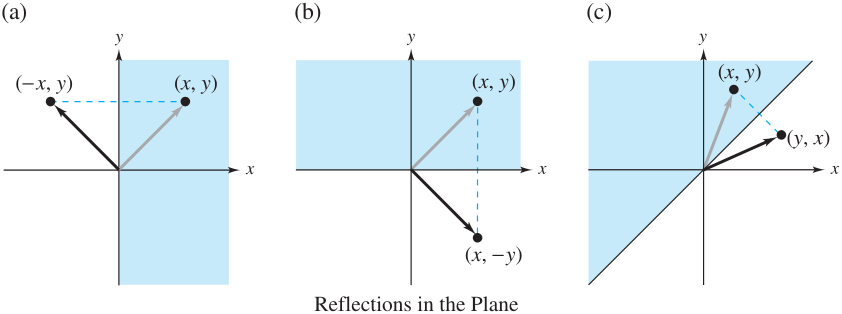
\includegraphics[width = 8cm]{images/reflect2d.png}
    \end{center}
    \textbf{Example 2. \textcolor{blue5}{Expansions and Contractions in the Plane}}
    
    \begin{center}
        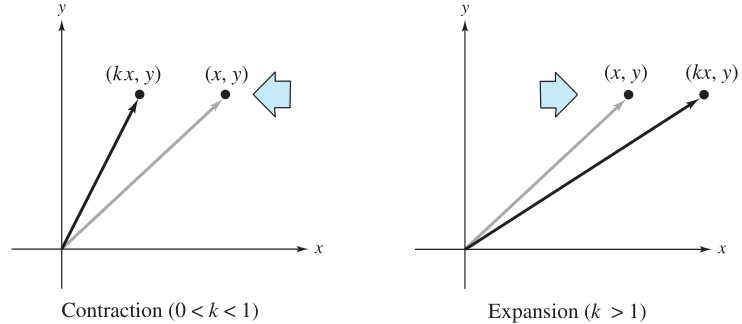
\includegraphics[width = 8cm]{images/expandX.png}
    \end{center}
    
    \begin{center}
        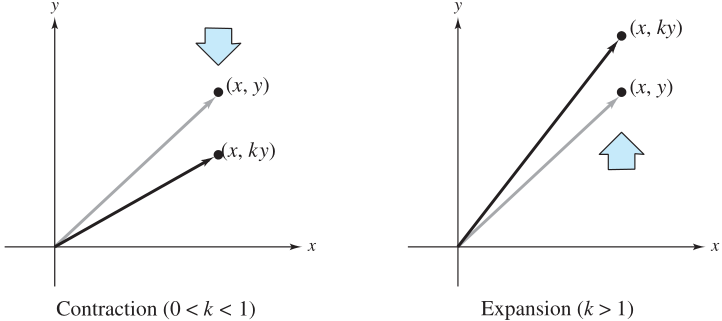
\includegraphics[width = 8cm]{images/expandY.png}
    \end{center}
    {\color{blue9} \rule{8cm}{0.3mm}}

    \textbf{Example 3. \textcolor{blue5}{Shears in the Plane}}

    \begin{minipage}{0.3\linewidth}
        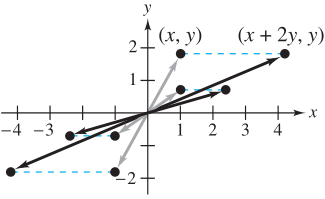
\includegraphics[width = 4cm]{images/shear2d.png}
    \end{minipage}
    \begin{minipage}{0.61\linewidth}
        The transformations defined by the following matrices are shears.
        \begin{equation*}
            \begin{array}{cccc}
                T(x,y) = (x + ky, y) & \quad & \quad & T(x,y) = (x, y + kx) \\
                \begin{bmatrix}
                    1 & k \\
                    0 & 1
                \end{bmatrix} \begin{bmatrix}
                    x \\ y
                \end{bmatrix} =
                \begin{bmatrix}[rr]
                    x + ky \\
                    y
                \end{bmatrix} & \quad & \quad & 
                \begin{bmatrix}
                    1 & 0 \\
                    k & 1
                \end{bmatrix} \begin{bmatrix}
                    x \\ y
                \end{bmatrix}
                    =
                \begin{bmatrix}[ll]
                    x \\
                    kx + y
                \end{bmatrix}
            \end{array}
        \end{equation*}
    \end{minipage}

    \section{Computer Graphics}
    
    \begin{minipage}{0.3\linewidth}
        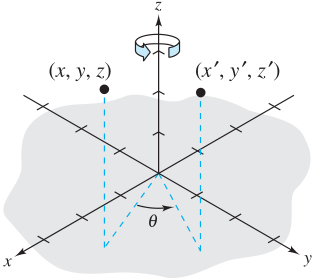
\includegraphics[width = 4cm]{images/rotatez3d.png}
    \end{minipage}
    \begin{minipage}{0.63\linewidth}
        Suppose we want to rotate the point $(x,y,z)$ counterclockwise about the $z$-axis through an angle $\theta$.
        \[ \begin{bmatrix}
            x' \\ y' \\ z'
        \end{bmatrix} = 
        \begin{bmatrix}[rrr]
            \cos{ \theta} & - \sin{ \theta } & 0 \\
            \sin{ \theta } & \cos{ \theta } & 0 \\
            0 & 0 & 1
        \end{bmatrix} \begin{bmatrix}
            x \\ y \\ z
        \end{bmatrix} = 
        \begin{bmatrix}
            x \cos{ \theta } - y \sin{ \theta } \\
            x \sin{ \theta } + y \cos{ \theta } \\
            z
        \end{bmatrix}\]
    \end{minipage}

    \textbf{Example 4. \textcolor{blue5}{Rotation About the $z$-Axis}}

    The 8 vertices of a rectangular box having sides of lengths 1, 2, and 3 are as follows.
    \begin{align*}
        V_1 &= (0,0,0), \quad & V_2 &= (1,0,0), \quad & V_3 &= (1,2,0), \quad & V_4 &= (0,2,0) \\
        V_5 &= (0,0,3), \quad & V_6 &= (1,0,3), \quad & V_7 &= (1,2,3), \quad & V_8 &= (0,2,3)
    \end{align*}
    Find the coordinates of the box when it is rotated $60^o$ counterclockwise about the $z$-axis.
    
    \begin{minipage}{0.3\linewidth}
        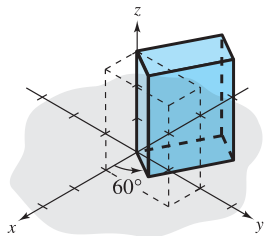
\includegraphics[width = 4cm]{images/60rotateZ.png}
    \end{minipage}
    \begin{minipage}{0.61\linewidth}
        The matrix that yields a rotation of $60^o$ is
        \[A = \begin{bmatrix}[rrr]
            \cos{ 60^o} & - \sin{60^o } & 0 \\
            \sin{ 60^o} & \cos{60^o } & 0 \\
            0 & 0 & 1
        \end{bmatrix} = \begin{bmatrix}
            1/2 & -\sqrt{3}/2 & 0 \\
            \sqrt{3}/2 & 1/2 & 0 \\
            0 & 0 & 1
        \end{bmatrix} \]
        And multiplying this matrix by each of the vertices.
    \end{minipage}

    {\color{blue9} \rule{10cm}{0.3mm}}
    
    \begin{Def}
        All three types of rotations are summarized as follows.
        \begin{align*}
            \textit{ \textcolor{blue5}{\footnotesize Rotation About the $x$-Axis} } & &
            \textit{ \textcolor{blue5}{\footnotesize Rotation About the $y$-Axis} } & &
            \textit{ \textcolor{blue5}{\footnotesize Rotation About the $z$-Axis} }\\
                \begin{bmatrix}
                    1 & 0 & 0 \\
                    0 & \cos{ \theta } & - \sin{ \theta } \\
                    0 & \sin{ \theta } & \cos{ \theta }
                \end{bmatrix}& &
                \begin{bmatrix}
                    \cos{ \theta } & 0 & \sin{ \theta } \\
                    0 & 1 & 0 \\
                    - \sin{ \theta } & 0 & \cos{ \theta }
                \end{bmatrix}& &
                \begin{bmatrix}
                    \cos{ \theta } & - \sin{ \theta } & 0 \\
                    \sin{ \theta } & \cos{ \theta } & 0 \\
                    0 & 0 & 1
                \end{bmatrix}
        \end{align*}
        \begin{center}
            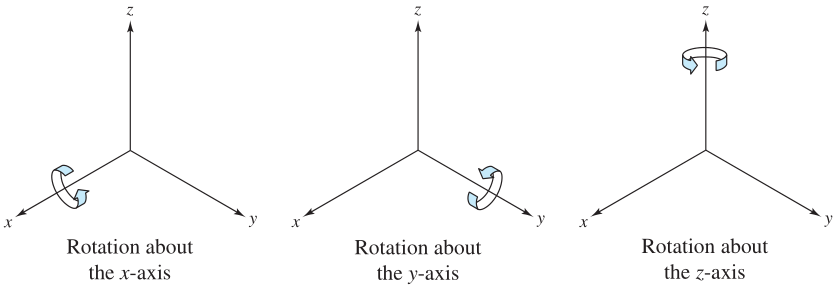
\includegraphics[width = 10cm]{images/rotatexyz.png}
        \end{center}
    \end{Def}
    \begin{minipage}{0.57\linewidth}
        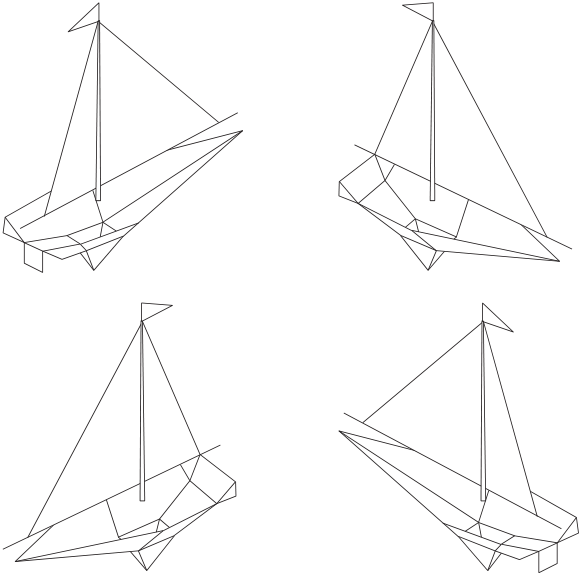
\includegraphics[width = 9cm]{images/graphic.png}
    \end{minipage}
    \begin{minipage}{0.4\linewidth}
        The use of computer graphics has become common among designers in many fields. By simply entering
        the \textbf{coordinates} that form the outline of an object into a computer, a designer can see the object before it is
        created.
    \end{minipage}

    














    
    
\end{document}
